\documentclass[12pt]{extarticle}
\usepackage[utf8]{inputenc}
\usepackage{graphicx}
\usepackage{fancyhdr}
\usepackage{geometry}
\usepackage{lipsum}
\usepackage{tocloft} % Para el índice
\usepackage{hyperref} % Para que los elementos referenciados sean clickables
\usepackage{amsmath}
\numberwithin{equation}{section}
\setlength{\jot}{14pt} % Para separar las líneas de ecuaciones
\usepackage{amssymb}
\usepackage{float} % Para colocar las imágenes y tablas

\usepackage{caption}
\usepackage{listings}
\usepackage{hyperref}
\captionsetup[lstlisting]{%
    aboveskip=14pt,   % espacio extra entre el código y la caption
    belowskip=12pt    % espacio extra después de la caption
}
\lstset{
    xleftmargin=.2\textwidth,
    xrightmargin=.2\textwidth
}
\renewcommand{\tableautorefname}{Table}
\renewcommand{\figureautorefname}{Figure}
\renewcommand{\equationautorefname}{Equation}
\renewcommand{\lstlistingname}{Algorithm}

% en el preámbulo
\usepackage{listings}
\usepackage{xcolor}
\lstset{
  language=Python,
  basicstyle=\ttfamily\scriptsize,
  keywordstyle=\color{blue},
  stringstyle=\color{teal},
  commentstyle=\color{gray}\itshape,
  numbers=left,
  numberstyle=\tiny,
  frame=none, % single para un recuadro negro
  captionpos=b,
  breaklines=true,
  showstringspaces=false
}

% Configuración de márgenes
\geometry{top=2.5cm, bottom=4cm, left=2.5cm, right=2.5cm}

\begin{document}

% Portada
\begin{titlepage}
    \centering
    
\includegraphics[width=0.35\textwidth]{images/Logo_comillas.png}\\[1cm] 
    {\Huge \textbf{GRADO EN INGENIERÍA}}\\[0.3cm]
    {\Huge \textbf{MATEMÁTICA E INTELIGENCIA}}\\[0.5cm]
    {\Huge \textbf{ARTIFICIAL}}\\[1.5cm]
    {\Huge \textbf{TRABAJO FIN DE GRADO}}\\[1.3cm]
    {\huge INTERPRETING NEURAL NETWORKS -}\\[0.4cm]
    {\huge DEVELOPING A METHODOLOGY FOR }\\[0.4cm]
    {\huge BANKING CASE STUDIES USING }\\[0.4cm]
    {\huge EXPLAINABLE AI}\\[0.4cm]
    \textbf{Autor: Javier Prieto Domínguez}\\[0.5cm]
    \textbf{Co-Director: David Alfaya Sanchez}\\[0.5cm]
    \textbf{Co-Director: Jaime Pizarroso Gonzalo}\\
    \raisebox {-2cm}[0cm][0cm]{\large Madrid, Junio}
    \vfill
\end{titlepage}

% Aumentar el espacio del encabezado para evitar que se solape
\setlength{\headheight}{2cm}  % Ajusta esto según el tamaño de la imagen

% Configuración del encabezado
\pagestyle{fancy}
\fancyhf{}
\fancyhead[L]{
\includegraphics[width=2cm]{images/Color_logo_comillas.png}} % A la izquierda
% \fancyhead[C]{\textbf{UNIVERSIDAD PONTIFICIA COMILLAS}}  % En el centro
% \fancyhead[R]{\textbf{ICAI}}  % A la derecha

% Texto en el encabezado
\fancyhead[C]{
    \hspace{2cm}
    \textbf{UNIVERSIDAD PONTIFICIA COMILLAS}\\
    \hspace{2cm}
    Escuela Técnica Superior de Ingeniería (ICAI)\\
    \hspace{2cm}
    Grado en Ingeniería Matemática e Inteligencia Artificial
}

% Página 2 Declaración de Responsabilidad
\newpage

{\fontsize{14}{18}\selectfont
    % Declaración o contenido de la página (texto justificado)
    Declaro, bajo mi responsabilidad, que el Proyecto presentado con el título \textbf{Interpreting Neural Networks - Developing a Methodology for Banking Case Studies Using Explainable AI} en la ETS de Ingeniería - ICAI de la Universidad Pontificia Comillas en el curso académico 2024/25 es de mi autoría, original e inédito y no ha sido presentado con anterioridad a otros efectos. \\
    
    El Proyecto no es plagio de otro, ni total ni parcialmente y la información que ha sido tomada de otros documentos está debidamente referenciada.
    
    \vspace{2cm}  % Espacio entre párrafos
    
    \noindent
    \makebox[\textwidth][s]{Fdo.: \textbf{Javier Prieto Domínguez} \hfill Fecha: 10/06/2025}

    
    \vspace{2cm}  % Espacio entre las firmas y la siguiente sección
    
    \begin{center}
        Autorizada la entrega del proyecto \\
        \vspace{1cm}
        \textbf{LOS DIRECTORES DEL PROYECTO}
    \end{center}
    
    \vspace{1cm}  % Espacio entre el título y la firma
    
    \noindent
    \makebox[\textwidth][s]{Fdo.: \textbf{David Alfaya Sánchez} \hfill Fecha: 10/06/2025}
    \noindent
    \makebox[\textwidth][s]{Fdo.: \textbf{Jaime Pizarroso Gonzalo} \hfill Fecha: 10/06/2025}
}

% Página 3 Agradecimientos
\newpage

{\fontsize{17}{20}\selectfont
    \begin{center}
        \textbf{AGRADECIMIENTOS}
    \end{center}
    % aqui
}

\newpage
\begin{abstract}
    Neural networks are increasingly employed in the banking sector for tasks ranging from credit scoring to fraud detection. Despite their powerful predictive capabilities, the opacity of neural network models poses significant challenges for their interpretability. This project aims to bridge the gap between complex neural network architectures and their practical interpretation by developing a comprehensive methodology utilizing state-of-the-art Explainable AI (XAI) techniques.
\end{abstract}

% Índice de la memoria
\newpage
\tableofcontents  % Esto genera el índice automáticamente
\thispagestyle{fancy}

% Comienza la memoria
\newpage
% \twocolumn

% Aumentar el espacio entre la línea y el número de página
\renewcommand{\footrulewidth}{0.4pt}  % Línea separadora en el pie de página
\setcounter{page}{1}  % Empezar la numeración de páginas desde la página 6
\fancyfoot[C]{
    \begin{center}
        \thepage
    \end{center}
}  % Mueve el número de página 0.5cm hacia abajo desde la línea
\setlength{\footskip}{0.8cm}  % Aumenta la distancia entre el contenido y 

%%%%%%%%%%%%%%%%%%%%%%%%%%%%%%%%%%%%%%%%%%%%%%%%%%%%%%%%
%%%% Introduction %%%%%%%%%%%%%%%%%%%%%%%%%%%%%%%%%%%%%%
%%%%%%%%%%%%%%%%%%%%%%%%%%%%%%%%%%%%%%%%%%%%%%%%%%%%%%%%
\section{Introduction}
Currently, the regulations many entities face on the use of AI are very restrictive. They must be able to "explain" the decisions made by their models to justify business decisions based on those AI systems~\cite{cohen2021black}. Today, the vast majority of them use models such as decision trees, random forests, and logistic regressions due to the lack of interpretability 
of bigger and more powerful models~\cite{ghatasheh2014business,pointofview}. The aim of this project is to provide a solution to solve two main problems. First, neural networks and larger models are considered ``black-box'' models, so we cannot fully understand the decision-making processes behind specific outputs, and therefore result useless when facing regulations. Secondly, we wish to give \emph{actionable} solutions for differentiable classification models, such as neural networks or logistic regressions, by identifying changes in input features that could alter the model output.\\
\\
In the context of banking and loan applications, for example, if a loan application is denied, the solution should provide actionable insights, such as ``reduce your debt by \$10,000 to qualify'' or ``increase your salary by \$5,000 to qualify.'' These are concrete changes in the individual's profile that can change the classification outcome. These \emph{explanations} or actionable changes are known as \emph{counterfactuals}~\cite{wachter2017counterfactual,guidotti2024counterfactual}. A counterfactual reveals what should have been different in an instance to observe a different outcome. These explanations are a clear and direct definition for local interpretability. It provides an insight into why a singular instance has been classified a certain way. For our specific case, our aim is not to solve or provide global interpretability, as the end user, or clients of a bank, do not need to know the reason a model behaves a certain way for the entire dataset.\\
\\
Our objective is to devise a novel counterfactual technique based on an \emph{optimal mathematical solution} to the problem, using optimization methods and the model's derivatives to find the minimal shift needed for a given instance to change its output. We propose a customizable solution in which the end user is able to weigh how easy or difficult is to change each of the original features.


\subsection{Estructura del Trabajo} %#TODO

%%%%%%%%%%%%%%%%%%%%%%%%%%%%%%%%%%%%%%%%%%%%%%%%%%%%%%%%
%%%% Related works %%%%%%%%%%%%%%%%%%%%%%%%%%%%%%%%%%%%%
%%%%%%%%%%%%%%%%%%%%%%%%%%%%%%%%%%%%%%%%%%%%%%%%%%%%%%%%
\section{Related works}
Research in counterfactual explanations often highlights a set of properties a good explanation should fulfill~\cite{guidotti2024counterfactual}. These are:
\begin{itemize}
  \item \textbf{Validity:} The counterfactual truly changes the classification outcome.
  \item \textbf{Minimality:} The counterfactual changes only the smallest set (or magnitude) of features.
  \item \textbf{Similarity:} The counterfactual remains close to the original instance by some distance metric.
  \item \textbf{Plausibility:} The counterfactual resembles realistic feature values found in the reference dataset.
  \item \textbf{Actionability:} The counterfactual only changes features that can realistically be altered (e.g., debt reduction but not age).
  \item \textbf{Diversity:} A set of counterfactuals should offer varied options for achieving the desired outcome.
\end{itemize}
Other desirable properties of the explanation \emph{itself} are
efficiency, which speaks to the speed of the method of returning the explanations; stability, if two instances are similar, their counterfactual explanations should be similar as well; and fairness, explanation remains valid even if sensitive attributes (e.g., ethnicity) were altered~\cite{guidotti2024counterfactual}.\\
\\
Counterfactual methods can be categorized by the strategy used to create the explanations. The main strategies include Optimization-based, Heuristic-based, Instance-based, and Decision-tree-based methods~\cite{guidotti2024counterfactual}. While optimization-based explainers usually have outstanding results in many of the individual properties highlighted above, they usually lack a good trade-off between all of them. Heuristic, instance and decision tree based methods are usually endogenous, meaning the counterfactual returned comes from the original dataset, which provides good results for plausibility and diversity, but not for similarity. On the other hand, optimization methods are in their majority exogenous, meaning they create a new sample based on the algorithm they follow, which usually performs good on minimality and similarity while possibly leaving other properties like plausibility and actionability unfulfilled. The current state-of-the-art does not yet include an explainer that fulfills all the desirable properties~\cite{guidotti2024counterfactual}.\\
\\
The task of finding an algorithm that fulfills all of the properties has been attempted in many papers. The most well-known technique in counterfactual space is WACH~\cite{wachter2017counterfactual}, one of the first papers to publish and propose these explanations. They propose a loss function, adopted by other explainers, consisting in a distance function and a cross-entropy loss, which they try to minimize with a common optimizer such as SGD~\cite{} or Adam~\cite{}. 


; ACTREC (Actionable Recourse)~\cite{ustun2019actionable} among the first to consider which features can be changed and which must remain fixed; DiCE~\cite{}, which generates a set of diverse counterfactuals for a single instance; or SGNCE~\cite{}, which guarantees the nearest counterfactual optimizing a mixed integer problem. Although XAI methods like LIME~\cite{ribeiro2016why} and SHAP~\cite{lundberg2017unified} exist, they tend to assign feature importance rather than produce clear, actionable changes in the input that could alter the classification. They both have adapted to the counterfactual world~\cite{,} but with little success~\cite{}.\\
\\

Our objective is to devise a novel counterfactual technique based on an \emph{optimal mathematical solution} to the problem, using optimization methods and the model's derivatives to find the minimal shift needed for a given instance to change its output, fitting into the optimization-based category. We not only fulfill this similarity to the original instance by minimizing a distance function, validity and plausibility are guaranteed as well with how the method works. Other features like minimality, actionability, and diversity are achieved through a set of weights that determine the decisions and inner workings of the method in every step. This gives the ability, to either the entity using the algorithm or the client, to determine which features are actually changeable and how difficult it is to change it.
\\


%%%%%%%%%%%%%%%%%%%%%%%%%%%%%%%%%%%%%%%%%%%%%%%%%%%%%%%%
%%%% Methodology %%%%%%%%%%%%%%%%%%%%%%%%%%%%%%%%%%%%%%%
%%%%%%%%%%%%%%%%%%%%%%%%%%%%%%%%%%%%%%%%%%%%%%%%%%%%%%%%
\section{Methodology}
The purpose of this project is to create a innovative XAI technique for differentiable models. We will initially restrict the analysis to differentiable models since the method requires the use of derivatives for optimization matters and for that, differentiability is needed. We will also assume that it is a binary classification model with a threshold This new technique, or method, falls into the Counterfactual Explanations family of XAI. As mentioned earlier in the motivation, a counterfactual reveals what should have been different in an instance to observe a diverse outcome.
\\

Following the definition of a counterfactual, and inspired by some of the main properties mentioned earlier, the innovative method aims to fulfill, or have, as many properties as possible. With the validity and similarity properties in mind, which refer to counterfactuals that succeed in changing the classification output with the minimum change needed, the mathematical optimization method of Lagrange multipliers comes up with a direct application to the problem. In this optimization method, it is possible to find local minimum (or maximum but it doesn’t apply to the problem) of a function with certain equation constraints. In the case of the counterfactual, we want to minimize the distance between the original instance and the new instance, subject to the condition of changing its classification output. This would fulfill both of the properties mentioned above. The equation with the Lagrangian multiplier becomes:

\[
\mathcal{L}(x, \lambda) = \; C(x, x_0) + \lambda \, \Bigl(M(x) - \theta \Bigr),
\]
where
\begin{itemize}
  \item $x$ is the new instance (the counterfactual) with m features,
  \item $x_0$ is the original instance,
  \item $C(\cdot)$ is a cost function (distance) measuring how far $x$ is from $x_0$,
  \item $M(\cdot)$ is the differentiable model, 
  \item $\theta$ is the threshold for changing the classification, and
  \item $\lambda$ is the Lagrange multiplier.
\end{itemize}
The cost function consists of a weighted cost function, 
whose values can be set to tailor the solution to the problem at hand. The problem we will be 
aiming to solve is related to loan applications, specifically how to “fool” the model, or what 
changes a person can make to get their application accepted instead of denied.

\subsection{Mathematical solution}
The minimum value of $\mathcal{L}$ is found when the partial derivatives 
w.r.t.\ $\mathbf{x}$ and $\lambda$ are equal to 0. This implies:
\begin{equation}\label{eq:deriv}
F(\mathbf{x}, \lambda) \;=\; \nabla \mathcal{L}(\mathbf{x}, \lambda) \;=\;
\begin{cases}
\nabla C(\mathbf{x}) \;-\;\lambda\,\bigl(\nabla M(\mathbf{x})\bigr) \;=\; 0, \\
-\,M(\mathbf{x})\;+\;\varepsilon\;=\;0.
\end{cases}
\end{equation}
\noindent
To solve this problem we will use the \emph{Newton-Raphson} method to solve this mathematical problem, ensuring we reach the optimal solution. Newton's methods are used to find the roots of a function, or the solution to the equation $f(x) = 0$. In optimization, with $f \in C^2$, we are trying to find the roots of $f'$, or the solutions to $f'(x) = 0$, known as critical points. These points can be minima, maxima or saddle points, but in the case of this problem we will try to find the minima of the function $f$. \\
\\
For this, Newton-Raphson’s method of optimization uses the first and second term of the Taylor expansion of the function to find that point iteratively~\cite{fliege2009newton}. For 1 dimension, or 1 variable, the update rule is $x_{k+1}=x_{k}-{\frac {f'(x_{k})}{f''(x_{k})}}$. As seen in \eqref{eq:deriv}, we have two variables, so the we have to use the generalization of the iterative scheme using the hessian as the second derivative. Thus, the new iterative scheme obtained becomes
\[
\bigl(\mathbf{x}_{n+1},\,\lambda_{n+1}\bigr)
\;=\;
\bigl(\mathbf{x}_n,\,\lambda_n\bigr)
\;-\;
\mathbf{H}^{-1}\!\bigl(\mathcal{L}(\mathbf{x}_n,\lambda_n)\bigr)
\;\cdot\;
\nabla\mathcal{L}\bigl(\mathbf{x}_n,\lambda_n\bigr).
\]
\noindent
If we set $F(\mathbf{x},\lambda) \;=\;\nabla \mathcal{L}(\mathbf{x},\lambda)$, 
the equation simplifies to
\[
\bigl(\mathbf{x}_{n+1},\,\lambda_{n+1}\bigr)
\;=\;
\bigl(\mathbf{x}_n,\,\lambda_n\bigr)
\;-\;
\mathbf{J}\!\bigl(F(\mathbf{x}_n,\lambda_n)\bigr)
\;\cdot\;
F\!\bigl(\mathbf{x}_n,\lambda_n\bigr),
\]
where
\[
\mathbf{J}\!\bigl(F(\mathbf{x}_n,\lambda_n)\bigr)
\;=\;
\begin{pmatrix}
H\!\bigl(C(\mathbf{x}_n)\bigr)\;-\;\lambda_n\,H\!\bigl(M(\mathbf{x}_n)\bigr) 
    & -\,\nabla M(\mathbf{x}_n)
\\[6pt]
-\,\nabla M(\mathbf{x}_n)
    & 0
\end{pmatrix}.
\]
\noindent
Above, $H(\cdot)$ denotes the Hessian (second derivative) with respect to $\mathbf{x}$, 
and $\nabla(\cdot)$ denotes the gradient (first derivative).\\
\\
A similar method of optimizing a loss function has been done in the past (BFGS \cite{papakonstantinou2009historical}), 
but due to the computational complexity of calculating second derivatives, most of the work has been with its approximations. In this case, we will employ a recently created system, called 
\emph{NeuralSens} \cite{neuralsens}, to calculate these second derivatives efficiently, 
eliminating the need for approximations.\\
\\
All of this will be implemented programmatically in \texttt{PyTorch}, using neural networks (or logistic regressions if there are no hidden layers), which, using activations like \emph{sigmoid} or \emph{tanh}, are at least twice-differentiable.\\
\\
Notwithstanding, this mathematical approach has some challenges. 
First, in some iterations of some datapoints, the hessian can become singular or ill-conditioned, meaning that the inverse does not exist or it is very big and the update step explode. This causes problems to the overall convergence of the method for that certain point. 
Second, many real-life datasets include variables like integer and categorical columns. The method works very well with continuous variables but it does not have a direct and easy solution for dealing with these column types.

\subsection{Singular Matrices}
As discussed, one of the main problems when taking this optimization-based generation is the possibility of singular or ill-conditioned Hessians. This can most tipically happen because of two main things. If we have two variables that have a high correlation, they most likely will have a very small eigenvalue, which means that the matrix could become ill-conditioned or even singular. This is very easily solved by performing a bit of exploratory data analysis and removing highly correlated variables. This is already a common practice in the data science world, so it is assumed that it should not produce any problems.

The second problem is harder to solve, and it is the one we will be discussing in this section. This problem is when the gradient of the model is very close to 0, or the model has a flat curvature around a particular input. This leads again to a small eigenvalue, and the matrix becomes ill-conditioned. We explored some techniques like using the pseudo-inverse, damping techniques or switching to first-order updates for the affected iterations, but the experiments were not successful.To mitigate this issue, we implement an alternative update strategy when this type of ill-conditioning in the Hessian is detected. 

The ulterior objective behind this method is to find a valid counterfactual, which ideally is a point close to the original with a different classification output. If the 

To solve this problem more robust solution is to reduce the dimensionality of the problem by focusing on a sub-Hessian matrix, which captures the curvature information only for a subset of sensitive features.


\subsection{Singular Matrices}

As discussed, one of the primary numerical challenges in optimization-based counterfactual generation stems from the possibility of encountering singular or ill-conditioned Hessians. These matrices, which are critical for the second-order optimization step, may not be invertible due to very small or zero eigenvalues, typically when gradients are close to zero or the model has a flat curvature around a particular input.

This leads to a natural question: \textit{Why can't the top-left element (or sub-block) of the Hessian matrix be singular or non-invertible?} In practice, it can be, especially when one or more partial derivatives vanish or show strong dependencies among variables. If the derivative of the model with respect to a specific feature is close to zero, this introduces a degeneracy in the Hessian and can render it non-invertible or very unstable numerically. This directly affects the convergence of Newton-like methods, as the step update becomes unreliable or undefined.

To mitigate this issue, we implement an alternative update strategy when ill-conditioning is detected. This involves using a pseudo-inverse, damping techniques, or switching to first-order updates for affected iterations. However, a more robust solution involves reducing the dimensionality of the problem by focusing on a sub-Hessian matrix, which captures the curvature information only for a subset of sensitive features.

This leads to the following updated step, derived using the sub-Hessian:

\[
x_{n+1} = x_n - \left( \nabla^2 L(x_n) \right)^{-1} \nabla L(x_n)
\]

where \( \nabla^2 L(x_n) \) is the Hessian of the loss function \( L \) at step \( x_n \), and \( \nabla L(x_n) \) is the gradient. If the full Hessian is ill-conditioned, we instead define a subspace \( \mathcal{S} \) of features with significant gradients and compute:

\[
x_{n+1}^{(\mathcal{S})} = x_n^{(\mathcal{S})} - \left( \nabla^2_{\mathcal{S}} L(x_n) \right)^{-1} \nabla_{\mathcal{S}} L(x_n)
\]

Here, \( \nabla^2_{\mathcal{S}} L(x_n) \) and \( \nabla_{\mathcal{S}} L(x_n) \) denote the Hessian and gradient restricted to the subspace \( \mathcal{S} \).

This sub-Hessian approach improves numerical stability while still leveraging second-order optimization where it matters most.


\subsection{Discrete features}
To address discrete variables, we found that imposing a regularizer to the distance function worked the best for the task. The regularizer is designed 
to take value 0 at the integer points. We explored different trigonometric funcions, such as sines and cosines with periods matching the integers, but some features were getting stuck on the maxima of that function, as it has derivative 0 as well and Newton's method is designed to find critical points in general. The function we finally proposed for solving the discrete challenge faced was
\begin{equation}
    tan(\pi * x)
\end{equation}
that looks something like
\begin{figure}[H]
    \centering
    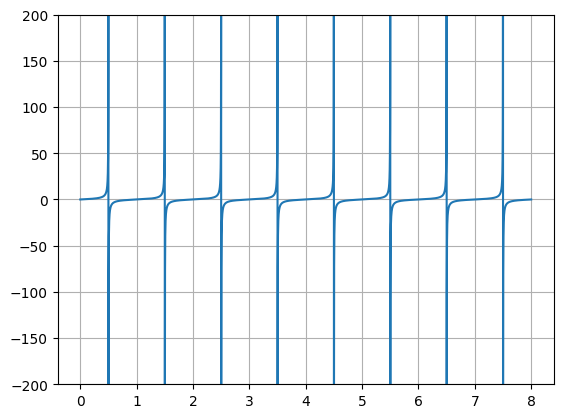
\includegraphics[width=0.6\textwidth]{images/integers}
    \caption{Tangent regularizer function}
    \label{fig:reg tan}
\end{figure}
\noindent
This function takes the value 0 in the integer points, but more importantly, they are saddle points, which are critical points in the newton's method. This means that iteratively, the features where the regularization is enforced will end up in one of those points, rather than in the possible optimum that could be a non-integer value.\\
\\


\subsection{Entrenamiento y Validación}

\section{Experimentos}
\subsection{Objetivos}
Lorem ipsum dolor sit amet, consectetur adipiscing elit, sed do eiusmod tempor incididunt ut labore et dolore magna aliqua. \autoref{eq:navier_stokes} % Podemos citar así para "Ecuación 5.4

\subsection{Conjunto de Datos}
Lorem ipsum dolor sit amet, consectetur adipiscing elit, sed do eiusmod tempor incididunt ut labore et dolore magna aliqua. \eqref{eq:navier_stokes} % Podemos citar así para "(5.4)"

\subsection{Configuración}
Lorem ipsum dolor sit amet, consectetur adipiscing elit, sed do eiusmod tempor incididunt ut labore et dolore magna aliqua. \eqref{eq:heat_b1} \eqref{eq:heat_b2}

\subsection{Análisis de Rendimiento}
Lorem ipsum dolor sit amet, consectetur adipiscing elit, sed do eiusmod tempor incididunt ut labore et dolore magna aliqua. \\

\begin{lstlisting}[caption={Entrenamiento de la red con Adam}, label={code:adam}]
import torch
import torch.nn as nn
import torch.optim as optim

model = MyNetwork()
optimizer = optim.Adam(model.parameters(), lr=1e-3)
criterion = nn.MSELoss()

for epoch in range(100):
    optimizer.zero_grad()
    outputs = model(inputs)
    loss = criterion(outputs, targets)
    loss.backward()
    optimizer.step()

\end{lstlisting}


\subsection{Visualización}
Lorem ipsum dolor sit amet, consectetur adipiscing elit, sed do eiusmod tempor incididunt ut labore et dolore magna aliqua.

\subsubsection{Graficas}
Lorem ipsum dolor sit amet, consectetur adipiscing elit, sed do eiusmod tempor incididunt ut labore et dolore magna aliqua.

\section{Resultados}
Lorem ipsum dolor sit amet, consectetur adipiscing elit, sed do eiusmod tempor incididunt ut labore et dolore magna aliqua.

\begin{equation}\label{eq:onda}
u_{tt} - c^2\,\Delta u = 0
\end{equation}

\begin{gather} % Si usamos align pone todas las ecuaciones alineadas por los =, hay que poner &= en todos los =
  u_t = k\,u_{xx} + f(x,t), \label{eq:heat_b1} \\
  u(0,x) = u_0(x), \nonumber\\
  u(t,0) = 0,\quad u(t,L)=0. \label{eq:heat_b2}
\end{gather}

\begin{subequations}\label{eq:navier_stokes} % salen (3.1a) y (3.1b)
\begin{gather} 
  \rho\bigl(u_t + u\cdot\nabla u\bigr) + \nabla p = \mu\nabla^2 u, \\
  \nabla\cdot u = 0.
\end{gather}
\end{subequations}


\section{Conclusiones y Trabajos Futuros}
Lorem ipsum dolor sit amet, consectetur adipiscing elit, sed do eiusmod tempor incididunt ut labore et dolore magna aliqua. \cite{}


\begin{thebibliography}{99}

\bibitem{wachter2017counterfactual}
S.~Wachter, B.~Mittelstadt, and C.~Russell.
\newblock Counterfactual Explanations without Opening the Black Box: Automated Decisions and the GDPR.
\newblock {\em SSRN Electronic Journal}, 2017.

\bibitem{guidotti2024counterfactual}
R.~Guidotti.
\newblock Counterfactual Explanations and How to Find Them: Literature Review and Benchmarking.
\newblock {\em Data Mining and Knowledge Discovery}, 38:2770--2824, 2024.

\bibitem{bodria2023benchmarking}
F.~Bodria, F.~Giannotti, R.~Guidotti, F.~Naretto, D.~Pedreschi, and S.~Rinzivillo.
\newblock Benchmarking and survey of explanation methods for black box models.
\newblock {\em Data Mining and Knowledge Discovery}, 37(5):1719--1778, 2023.

\bibitem{ustun2019actionable}
B.~Ustun, A.~Spangher, and Y.~Liu.
\newblock Actionable Recourse in Linear Classification.
\newblock {\em Proceedings of KDD '19}, 2019.

\bibitem{ribeiro2016why}
M.~T. Ribeiro, S.~Singh, and C.~Guestrin.
\newblock ``Why Should I Trust You?'': Explaining the Predictions of Any Classifier.
\newblock {\em arXiv preprint arXiv:1602.04938}, 2016.

\bibitem{lundberg2017unified}
S.~Lundberg and S.-I. Lee.
\newblock A Unified Approach to Interpreting Model Predictions.
\newblock {\em arXiv preprint arXiv:1705.07874}, 2017.

\bibitem{cohen2021black}
S.~N. Cohen, D.~Snow, and L.~Szpruch.
\newblock Black-Box Model Risk in Finance.
\newblock {\em SSRN Electronic Journal}, 2021.

\bibitem{ghatasheh2014business}
N.~Ghatasheh.
\newblock Business analytics using random forest trees for credit risk prediction: a comparison study.
\newblock {\em International Journal of Advanced Science and Technology}, 72:19--30, 2014.

\bibitem{pointofview}
Anonymous.
\newblock Point of View: Using Random Forest for credit risk models (Machine learning and Credit Risk: a suitable marriage?), 2019.

\bibitem{neuralsens}
J.~Pizarroso, J.~Portela, and A.~Mu\~noz.
\newblock NeuralSens: Sensitivity Analysis of Neural Networks.
\newblock {\em Journal of Statistical Software}, 102(7):1--36, 2022.

\bibitem{fliege2009newton}
J.~Fliege, L.~M.~G. Drummond, and B.~F. Svaiter.
\newblock Newton's Method for Multiobjective Optimization.
\newblock {\em SIAM Journal on Optimization}, 20(2):602--626, 2009.

\bibitem{papakonstantinou2009historical}
J.~M. Papakonstantinou.
\newblock Historical Development of the BFGS Secant Method and its Characterization Properties.
\newblock 2009.

\bibitem{kaggleLoan1}
\newblock H, M.~Y. (2022). Loan default dataset. Kaggle. 
\newblock \url{https://www.kaggle.com/datasets/yasserh/loan-default-dataset}.

\bibitem{kaggleLoan2}
\newblock Dutta, G. (2020). Loan defaulter. Kaggle. 
\newblock \url{https://www.kaggle.com/datasets/gauravduttakiit/loan-defaulter/data}.

\bibitem{kaggleLoan3}
\newblock Coursera. Data Science Coding Challenge: Loan Default Prediction. 
\newblock \url{https://www.coursera.org/projects/data-science-coding-challenge-loan-default-prediction}.

\end{thebibliography}


\end{document}




